% AER E 361 Mission Report Template
% Spring 2023
% Template created by Yiqi Liang and Professor Matthew Nelson

% Document Configuration DO NOT CHANGE
\documentclass[12 pt]{report}
% --------------------LaTeX Packages---------------------------------
% The following are packages that are used in this report.
% DO NOT CHANGE ANY OF THE FOLLOWING OR YOUR REPORT WILL NOT COMPILE
% -------------------------------------------------------------------

\usepackage{hyperref}
\usepackage{parskip}
\usepackage{titlesec}
\usepackage{titling}
\usepackage{graphicx}
\usepackage{graphviz}
\usepackage[T1]{fontenc}
\usepackage{titlesec, blindtext, color} %for LessIsMore style
\usepackage{tcolorbox} %for references box
\usepackage[hmargin=1in,vmargin=1in]{geometry} % use 1 inch margins
\usepackage{float}
\usepackage{tikz}
\usepackage{svg} % Allows for SVG Vector graphics
\usepackage{textcomp, gensymb} %for degree symbol
\hypersetup{
	colorlinks=true,
	linkcolor=blue,
	urlcolor=cyan,
}
\usepackage{biblatex}
\addbibresource{lab-report-bib.bib}
\usepackage{amsmath}
\usepackage{listings}
\usepackage{multicol}
\usepackage{array}

\usepackage{hologo} %KYR: for \BibTeX
%\usepackage{algpseudocode}
%\usepackage{algorithm}
% This configures items for code listings in the document
\usepackage{xcolor}

\usepackage{fancyhdr} % Headers/Footers
\usepackage{siunitx} % SI units
\usepackage{csquotes} % Display Quote
\usepackage{microtype} % Better line breaks

\definecolor{commentsColor}{rgb}{0.497495, 0.497587, 0.497464}
\definecolor{keywordsColor}{rgb}{0.000000, 0.000000, 0.635294}
\definecolor{stringColor}{rgb}{0.558215, 0.000000, 0.135316}
\definecolor{mygreen}{rgb}{0,0.6,0}
\definecolor{mygray}{rgb}{0.5,0.5,0.5}
\definecolor{mymauve}{rgb}{0.58,0,0.82}

\lstdefinestyle{customc}{
  belowcaptionskip=1\baselineskip,
  breaklines=true,
  frame=L,
  xleftmargin=\parindent,
  language=C,
  showstringspaces=false,
  basicstyle=\footnotesize\ttfamily,
  keywordstyle=\bfseries\color{green!40!black},
  commentstyle=\itshape\color{purple!40!black},
  identifierstyle=\color{blue},
  stringstyle=\color{orange},
 }

 \lstset{ %
  backgroundcolor=\color{white},   % choose the background color; you must add \usepackage{color} or \usepackage{xcolor}
  basicstyle=\footnotesize,        % the size of the fonts that are used for the code
  breakatwhitespace=false,         % sets if automatic breaks should only happen at whitespace
  breaklines=true,                 % sets automatic line breaking
  captionpos=b,                    % sets the caption-position to bottom
  commentstyle=\color{commentsColor}\textit,    % comment style
  deletekeywords={...},            % if you want to delete keywords from the given language
  escapeinside={\%*}{*)},          % if you want to add LaTeX within your code
  extendedchars=true,              % lets you use non-ASCII characters; for 8-bits encodings only, does not work with UTF-8
  frame=tb,	                   	   % adds a frame around the code
  keepspaces=true,                 % keeps spaces in text, useful for keeping indentation of code (possibly needs columns=flexible)
  keywordstyle=\color{keywordsColor}\bfseries,       % keyword style
  language=Python,                 % the language of the code (can be overrided per snippet)
  otherkeywords={*,...},           % if you want to add more keywords to the set
  numbers=left,                    % where to put the line-numbers; possible values are (none, left, right)
  numbersep=8pt,                   % how far the line-numbers are from the code
  numberstyle=\tiny\color{commentsColor}, % the style that is used for the line-numbers
  rulecolor=\color{black},         % if not set, the frame-color may be changed on line-breaks within not-black text (e.g. comments (green here))
  showspaces=false,                % show spaces everywhere adding particular underscores; it overrides 'showstringspaces'
  showstringspaces=false,          % underline spaces within strings only
  showtabs=false,                  % show tabs within strings adding particular underscores
  stepnumber=1,                    % the step between two line-numbers. If it's 1, each line will be numbered
  stringstyle=\color{stringColor}, % string literal style
  tabsize=2,	                   % sets default tabsize to 2 spaces
  title=\lstname,                  % show the filename of files included with \lstinputlisting; also try caption instead of title
  columns=fixed                    % Using fixed column width (for e.g. nice alignment)
}

\lstdefinestyle{customasm}{
  belowcaptionskip=1\baselineskip,
  frame=L,
  xleftmargin=\parindent,
  language=[x86masm]Assembler,
  basicstyle=\footnotesize\ttfamily,
  commentstyle=\itshape\color{purple!40!black},
}

\lstset{escapechar=@,style=customc}

\titlelabel{\thetitle.\quad}

% From here on out you can start editing your document
\newcommand{\subtitle}[1]{%
  \posttitle{%
    \par\end{center}
    \begin{center}\LARGE#1\end{center}
    \vskip0.5em}%
}

\title{\textbf{Iowa State University
\\{\Large Aerospace Engineering}}}
\subtitle{AER E 322 Lab 01\\
		  Practice Experiment and Data Analysis}
\author{Matthew Mehrtens, Peter Mikolitis, and Natsuki Oda}

\newcommand{\etal}{\textit{et al}., }
\newcommand{\ie}{\textit{i}.\textit{e}., }
\newcommand{\eg}{\textit{e}.\textit{g}., }

% Define the headers and footers
\setlength{\headheight}{70.63135pt}
\geometry{head=70.63135pt, includehead=true, includefoot=true}
\fancypagestyle{plain}{
	\fancyhead{}\fancyfoot{} % clears the headers/footers
	\fancyhead[L]{\textbf{AER E 322}}
	\fancyhead[C]{\textbf{Aerospace Structures Laboratory Report}\\
					 \textbf{Lab 01 Practice Experiment and Data Analysis}\\
					 Section 4 Group 2\\
					 Matthew Mehrtens, Peter Mikolitis, and Natsuki Oda\\
					 \today}
	\fancyhead[R]{\textbf{Spring 2023}}
	\fancyfoot[C]{\thepage}
}
\pagestyle{fancy}
\fancyhead{}\fancyfoot{} % clears the headers/footers
\fancyhead[L]{\textbf{AER E 322}}
\fancyhead[C]{\textbf{Aerospace Structures Laboratory Report}\\
			  \textbf{Lab 01 Practice Experiment and Data Analysis}\\
			  Section 4 Group 2\\
			  Matthew Mehrtens, Peter Mikolitis, and Natsuki Oda\\
			  \today}
\fancyhead[R]{\textbf{Spring 2023}}
\fancyfoot[C]{\thepage}

\begin{document}
\maketitle
\tableofcontents

\chapter{Pre-Lab} \label{pre-lab}
\section{Introduction} \label{introduction}
Aircraft wings undergo oscillations and other random forces while in flight. This lab replicates and analyzes some of the forces and oscillations a wing will experience in flight while also serving as an introduction to the PASCO tool kits and data processing. To simulate the wing, we used a cantilevered aluminum beam, and to generate and measure the oscillations, we used a PASCO tool kit---specifically the PASCO wave driver, displacement sensor and motion sensor. There were three rounds of testing; each additional round of testing introduced a new variable into the beam movement that changed the shape of the data. The data was collected using the PASCO tool kit and software provided. After the lab, we analyzed and processed the data in Python to how each variable effected the oscillation of the beam.

\section{Objectives} \label{objectives}
During this lab, our primary objectives were to:
\begin{enumerate}
	\item Learn how to record data under dynamic conditions and analyze or post-process the data.
	\item Observe approximately how a common aerospace structural material might respond to oscillatory forces.
	\item Gain familiarity with the PASCO tool kit and the PASCO Capstone software.
\end{enumerate}

\section{Hypothesis} \label{hypothesis}
\subsection{Test 1} \label{hypothesis-test_1}
We predict this test will provide the cleanest data of the three tests. Since the only force acting on the beam should be from the wave driver, we expect the displacement graph to shown a uniform and steady wave---matching the oscillations of the wave driver. The data from this test should closely match the oscillations of an airplane wing in very steady flight.

\subsection{Test 2} \label{hypothesis-test_2}
This test adds a spring with a hanging weight to the cantilevered beam. Due to the oscillations of the spring-weight system, we expect to see sudden highs and lows in the data corresponding with when the spring is in compression or tension respectively. The data from this test should demonstrate the oscillations of the wing in steady flight if there is an additional oscillatory or vibrational force simultaneously acting on the wing.

\subsection{Test 3} \label{hypothesis-test_3}
This test is similar to Test \num{2} (see Section \ref{hypothesis-test_2}) except a third significant force has been introduced. Due to the addition of arbitrary impulses being applied by hand to the free end of the beam, we expect the data to show large peaks and dips in the data correlated with the timing of the impulses. The data from this test should demonstrate the oscillations of real flight as described in Section \ref{hypothesis-test_2} but also how the wing might react during periods of high turbulence where sudden, large impulses may act on the wing.

\chapter{Lab Work} \label{lab_work}
\section{Variables} \label{variables}
\subsection{Independent Variables} \label{variables-independent_variables}
\subsubsection{Wave Driver Frequency} \label{variables-independent_variables-wave_drive_frequency}
The frequency of the wave generated by the PASCO wave driver.

\subsubsection{Wave Driver Amplitude} \label{variables-independent_variables-wave_driver_amplitude}
The maximum voltage the wave driver will use when oscillating, proportional to the displacement of the wave driver arm.

\subsubsection{Sampling Frequency} \label{variables-independent_variables-sampling_frequency}
The time intervals at which the PASCO motion sensor or displacement sensor poll the position or displacement of the beam. Sensor with a higher sampling frequency will collect more data in the same amount of time.

\subsubsection{Smoothing Span} \label{variables-independent_variables-smoothing_span}
The number of elements after a given element used to calculate a rolling mean while data processing. A small smoothing span will better preserve the shape of the data; whereas, a larger smoothing span will better reduce noise and outliers.

\subsubsection{Time} \label{variables-independent_variables-time}
Each test was run for exactly \qty{15}{\s}, measured in \qty{0.01}{\s} intervals.

\subsection{Dependent Variables} \label{variables-dependent_variables}
\subsubsection{Displacement/Position} \label{variables-dependent_variables-displacement-position}
The change in location of the cantilevered beam from its equilibrium position, measured closer to the free end along a perpendicular vertical axis.

\subsubsection{Best Fit Curve} \label{variables-dependent_variablesbest_fit_curve}
The line of best fit or fit curve is a normalized curve matching the raw or smoothed data and depends on the shape and magnitude of the displacement data.

\section{Work Assignments} \label{work_assignments}
Refer to Table \ref{table:work_assignments} for the distribution of work during this lab.

\begin{table}[!ht]
\caption{Work assignments for AER E 322 Lab 01.}
\begin{center}
	\begin{tabular}{| c | c | c | c |}
		\hline
		\multicolumn{1}{| c |}{\textbf{Task}} & \textbf{Matthew} & \textbf{Peter} & \textbf{Natsuki} \\
		\hline
		\multicolumn{4}{| c |}{\textit{Lab Work}} \\
		\hline
		Date Recording & & X & \\
		\hline
		Exp. Setup & X & & \\
		\hline
		Exp. Work & & & X \\
		\hline
		Exp. Clean-Up & X & X & X \\
		\hline
		\multicolumn{4}{| c |}{\textit{Data Processing}} \\
		\hline
		Data Import & X & & \\
		\hline
		Smoothing & X & X & \\
		\hline
		Line of Best Fit & X & X & X\\
		\hline
		\multicolumn{4}{| c |}{\textit{Report}} \\
		\hline
		Introduction & & & X \\
		\hline
		Objectives & & X & \\
		\hline
		Hypothesis & X & & \\
		\hline
		Variables & & X & \\
		\hline
		Materials & & X & \\
		\hline
		Apparatus & & X & \\
		\hline
		Procedures & X & & \\
		\hline
		Data & X & & \\
		\hline
		Analysis & X & X & X \\
		\hline
		Conclusion & & & X \\
		\hline
		References & & & X \\
		\hline
		Appendix & & & X \\
		\hline
		Revisions & X & X & X \\
		\hline
		Editing & X & & \\
		\hline
	\end{tabular}
\end{center}
\label{table:work_assignments}
\end{table}

\section{Materials} \label{materials}
The materials required for this lab include: cantilever aluminum beam, spring, weight, Styrofoam pad, tape, round point-tip ``needle'' displacement sensor, C-clamps, wooden 2''x4'', bench vice, string, computer with PASCO Capstone software, clamp stand with clamps, PASCO 850 Universal Interface, PASCO mechanical wave driver, and a PASCO non-contact motion sensor.

\section{Apparatus} \label{apparatus}
Figure \ref{fig:lab_apparatus} shows the fully assembled lab apparatus. For Test \num{1}, the weight was removed from the spring. For Tests \num{2} and \num{3}, the weight was added back to the apparatus and the displacement sensor---the needle-like device on top of the beam---was removed.

\begin{figure}[htbp]
\centering
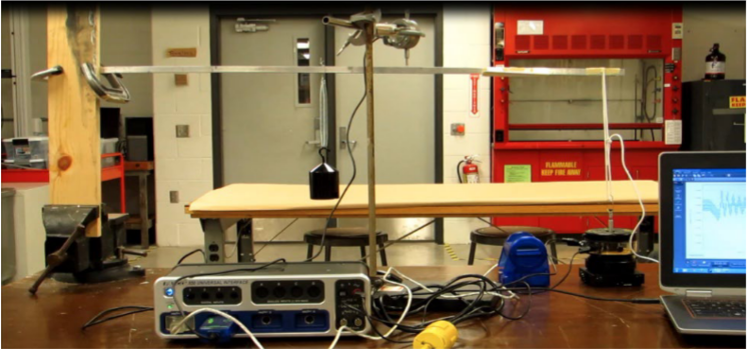
\includegraphics[width=6in]{images/Lab_Apparatus}
\caption{Lab apparatus completely set up, including the spring, weight, and displacement sensor. Image from the \textit{Lab 1 Practice Experiment and Data Analysis} manual \cite{lab_procedures}. Copyright 2023 by Thomas Chiou.}
\label{fig:lab_apparatus}
\end{figure}

As shown in Figure \ref{fig:lab_apparatus}, the left side of the beam is fixed to the board and the right side is attached to the wave driver with string. The rectangular, gray box in the foreground is the PASCO 850 Universal Interface, and the blue device in the midground is the motion sensor. The motion sensor must be positioned directly underneath the piece of white foam taped to the bottom of the beam with at least \qty{15}{\cm} between the sensor and the foam.

\section{Procedures} \label{procedures}
\subsection{Setup} \label{procedures-setup}
Assemble the apparatus as described in Section \ref{apparatus}. Ensure that the styrofoam reflector plate is at least \qty{15}{\cm} away from the motion sensor before running any tests. Launch the PASCO Capstone software, and turn on the PASCO 850 Universal Interface. Check that both the ``needle'' displacement sensor and motion sensors are recognized by the software. Once the sensors are recognized, configure the software to display two graphs ``by selecting the corresponding icon from the on-screen template'' \cite{lab_procedures}. Next, click on each axis to label the graphs, and set the y-label of the displacement sensor graph to ``displacement'' and ``position'' for the motion sensor graph. For both graphs, the x-label will be ``time''. Refer to Figure \ref{fig:pasco_main_page} to see how the graph layout should look.

\begin{figure}[htbp]
\centering
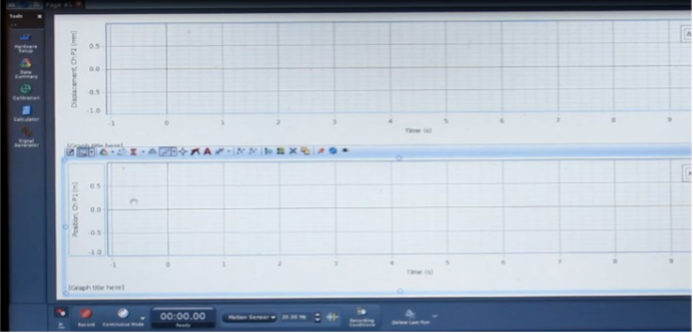
\includegraphics[width=5in]{images/PASCO_Main_Page}
\caption{The graph screen of the PASCO Capstone software fully configured for this lab. Image from the \textit{Lab 1 Practice Experiment and Data Analysis} manual \cite{lab_procedures}. Copyright 2023 by Thomas Chiou.}
\label{fig:pasco_main_page}
\end{figure}

Set up the wave driver by clicking the ``Signal Generator'' icon on the left-side of the screen.  Set the waveform to ``Sine'', sweep type to ``Off'', frequency to \qty{10}{\hertz}, amplitude to \qty{10}{\volt}, and select ``Auto'' at the bottom of the window. For reference, compare your ``Signal Generator'' window to Figure \ref{fig:wave_driver_setup}.

\begin{figure}[htbp]
\centering
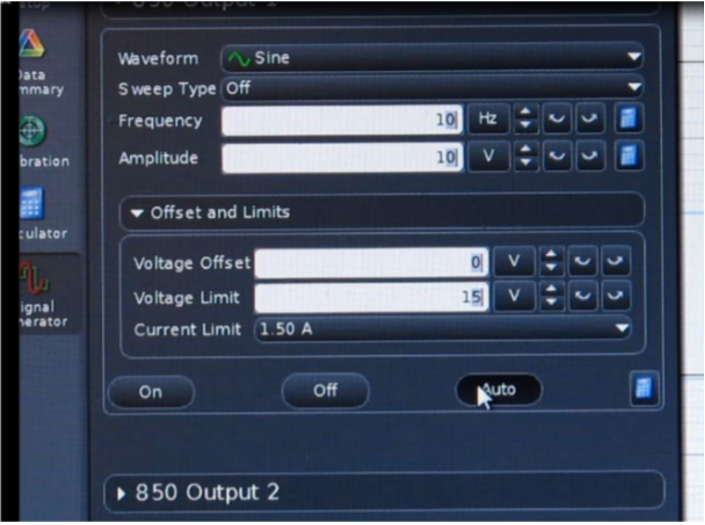
\includegraphics[width=4in]{images/Wave_Driver_Setup}
\caption{The wave driver or ``Signal Generator'' configuration window. Image from the \textit{Lab 1 Practice Experiment and Data Analysis} manual \cite{lab_procedures}. Copyright 2023 by Thomas Chiou.}
\label{fig:wave_driver_setup}
\end{figure}

Next, at the bottom of the screen select ``Recording Condition'', then select ``Stop Condition''. Set ``Condition Type'' to ``Time Based'', and set the time to \qty{15}{\s}. The ``Recording Condition'' window will look similar to Figure \ref{fig:stop_conditions}. 

\begin{figure}[htbp]
\centering
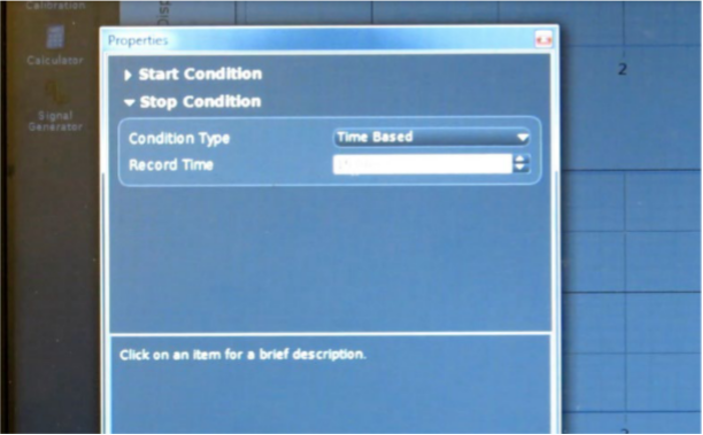
\includegraphics[width=4in]{images/Stop_Conditions}
\caption{The ``Stop Conditions'' configuration window. Image from the \textit{Lab 1 Practice Experiment and Data Analysis} manual \cite{lab_procedures}. Copyright 2023 by Thomas Chiou.}
\label{fig:stop_conditions}
\end{figure}

At the bottom of the screen, select ``Motion Sensor'', and set the sampling frequency to \qty{100}{\hertz}. The sensor can be zeroed by selecting the icon to the right of the sampling frequency field. Use the same process to set up the displacement sensor, except set the sampling frequency to \qty{5}{\hertz}. To zero the displacement sensor, click the physical O/I button on the sensor. The sensors should be zeroed before each round of testing.

Finally, navigate through the following menus: ``Data Summary'' icon on the left column of the screen $\rightarrow$ Motion Sensor $\rightarrow$ Position (m) $\rightarrow$ select the gear symbol $\rightarrow$ Numerical Format $\rightarrow$ change Number Style to Significant Figures $\rightarrow$ set the Number of Significant Figures to \num{5}. Follow the exact same process for the displacement sensor.

\subsection{Test 1} \label{procedures-test_1}
For Test \num{1}, we will only utilize the wave driver. Take the hanging weight off the beam before starting and remain clear of the apparatus during operation. Ensure the displacement sensor is making good contact with the beam and approximately halfway depressed. Check the motion sensor is directly under the styrofoam reflector plate with at least \qty{15}{\cm} of buffer. The string that attaches the beam to the axle socket of the wave driver should be taut. Lastly, double-check that the connector tip of the wave driver ``is firmly seated inside the axle socket'' \cite{lab_procedures}. Zero both sensors before running the test, then, in the PASCO Capstone software, click ``Record'' to run the test. Let the test run for the entire \qty{15}{\s} duration. 

\subsection{Test 2} \label{procedures-test_2}
Before beginning Test \num{2}, remove the displacement sensor from the beam and add the hanging weight to the spring. Begin the test as described in Section \ref{procedures-test_1}. As the test begins, a group member will pull the weight down and release it, allowing the spring-weight system to oscillate for the duration of the test. Be careful not to pull the weight down too hard.

\subsection{Test 3} \label{procedures-test_3}
For Test \num{3}, leave the apparatus as it was configured for Test \num{2} in Section \ref{procedures-test_2}. Start the test as described in Section \ref{procedures-test_1}. After beginning the test, in addition to pulling down and releasing the hanging weight, a group member will randomly tap the free end of the cantilevered beam up or down every \qtyrange{2}{3}{\s}for the duration of the test.

\subsection{Cleanup} \label{procedures-cleanup}
Using the ``File'' menu in the PASCO Capstone software, save the experiment data to a \texttt{.txt} or \texttt{.csv} file. Transfer the data to a flash drive for post-processing and analysis.

\section{Data} \label{data}
All data analysis was done with Python. The following packages were used for importing, smoothing, and processing the data:

\begin{itemize}
	\item \texttt{pandas} (\url{https://pandas.pydata.org/})
	\item \texttt{numpy} (\url{https://numpy.org/})
	\item \texttt{matplotlib} (\url{https://matplotlib.org/})
	\item \texttt{scipy} (\url{https://scipy.org/})
\end{itemize}

The data was in a \text{.csv} format which the \texttt{pandas} Python package had no difficulty importing and parsing. To smooth the data, we used the \href{https://pandas.pydata.org/pandas-docs/stable/reference/api/pandas.DataFrame.rolling.html}{\texttt{pandas.DataFrame.rolling()}} and \href{https://pandas.pydata.org/pandas-docs/stable/reference/api/pandas.DataFrame.mean.html}{\texttt{pandas.DataFrame.mean()}} functions. The \texttt{.rolling()} function selects a subset of the elements, and the \texttt{.mean()} function calculates the mean of that subset. See Listing \ref{code:smooth_df} for the function from our Python script that smoothed the data.

\lstinputlisting[label={code:smooth_df}, caption={The \texttt{smooth{\textunderscore}df()} function from our Python data processing script. This function smooths a \href{https://pandas.pydata.org/pandas-docs/stable/reference/api/pandas.DataFrame.html}{\texttt{pandas.DataFrame}} object once or in multiple passes as defined by the \texttt{smooth} argument.}, language=Python, firstline=160, lastline=170]{src/Lab-01-Analysis.py}

To generate the line of best fit, we first observed that the data in our graphs looked generally sinusoidal. To generate and graph a sinusoidal line of best fit, our best option was to use the \href{https://docs.scipy.org/doc/scipy/tutorial/optimize.html}{\texttt{scipy.optimize()}} function, but since the frequency of the beams displacement curve varied due to the forces we were applying to it---especially in Test \num{2} and Test \num{3}---the \texttt{scipy.optimize()} function struggled to accurately generate an appropriate line of best fit. Our final solution for generating the line of best fit involved using the \texttt{scipy.optimize()} function and the \href{https://numpy.org/doc/stable/reference/generated/numpy.fft.fftfreq.html}{\texttt{numpy.fft.fftfreq()}} and \href{https://numpy.org/doc/stable/reference/generated/numpy.fft.fft.html}{\texttt{numpy.fft.fft()}} functions which performs a \href{https://en.wikipedia.org/wiki/Fast_Fourier_transform}{Fast Fourier Transform} (FFT) on a \href{https://numpy.org/doc/stable/reference/generated/numpy.array.html}{\texttt{numpy.array}} object. See Listing \ref{code:sin_lobf} for our implementation of the sinusoidal line of best fit function.

\lstinputlisting[label={code:sin_lobf}, caption={The \texttt{sin{\textunderscore}lobf()} function from our Python data processing script. This function generates a sinusoidal line of best fit for data that is generally sinusoidal. It uses an FFT algorithm from the \texttt{scipy} package and an optimization function from the \texttt{numpy} package. The function was modified from unsym's post on StackOverflow \cite{sin_lobf}.}, language=Python, firstline=174, lastline=197]{src/Lab-01-Analysis.py}

We also tested using a piece-wise line of best fit generator, \ie the line of best was generated for smaller consecutive domains rather than the entire \qtyrange{0}{15}{\s} of data. The graphs generated using this method can be found in Appendix \ref{piece-wise_lobf_graphs}. The entirety of the data processing script is shown in Appendix \ref{lab-01-analysis.py}.

The following sections discuss the data from Tests \num{1}--\num{3}. For conciseness, only the most pertinent graphs are discussed below. All the graphs are included in Appendix \ref{graphs} for reference.

\subsection{Test 1} \label{data-test_1}
Shown in Figures \ref{fig:run_1-raw-zoomed} and \ref{fig:run_1-smoothed-zoomed} is the raw data and smoothed data respectively for Test \num{1}. The raw data shows the measurements from the displacement sensor and the motion sensor. The smoothed data omits the raw data from the displacement sensor.

The smoothed data was generated using a two-pass rolling mean algorithm. The first pass used a window of \num{5} and the second pass used a window of \num{3}. For clarity, only the data from \qtyrange{5}{8}{\s} is shown in Figures \ref{fig:run_1-raw-zoomed} and \ref{fig:run_1-smoothed-zoomed}.

\begin{figure}[htbp]
    \centering
    \begin{minipage}{0.45\textwidth}
        \centering
        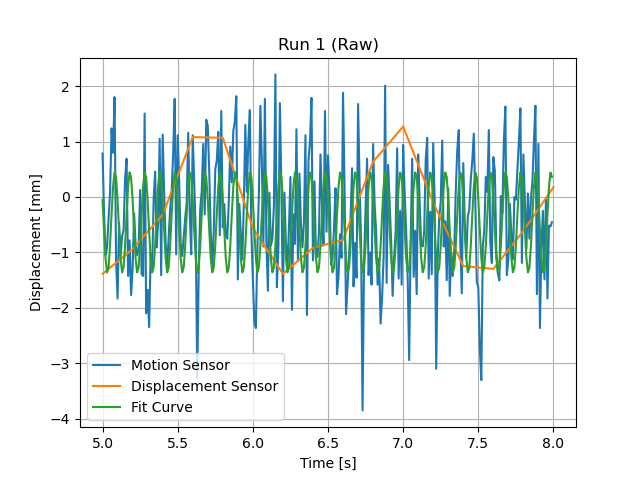
\includegraphics[width=1.0\textwidth]{images/Graphs/Run_1-Raw-Zoomed} % first figure itself
        \caption{Raw data from Test \num{1}, zoomed to only show \qtyrange{5}{8}{\s}.}
        \label{fig:run_1-raw-zoomed}
    \end{minipage}\hfill
    \begin{minipage}{0.45\textwidth}
        \centering
        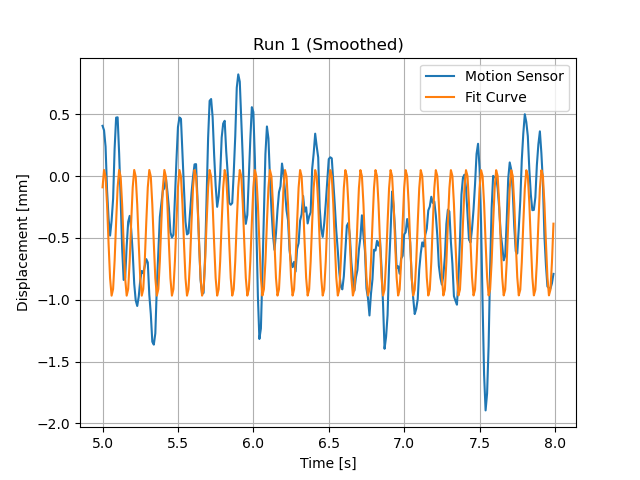
\includegraphics[width=1.0\textwidth]{images/Graphs/Run_1-Smoothed-Zoomed} % second figure itself
        \caption{Smoothed data from Test \num{1}, zoomed to only show \qtyrange{5}{8}{\s}.}
        \label{fig:run_1-smoothed-zoomed}
    \end{minipage}
\end{figure}

From these graphs, it is clear the displacement sensor's polling rate was too slow. In retrospect, the reason is clear. As shown from Figure \ref{fig:run_1-smoothed-zoomed} and as described in Section \ref{procedures-setup}, the wave driver was forcing the beam to oscillate at a rate of approximately \qty{10}{\hertz}, but the polling rate of the displacement sensor was \qty{5}{\hertz}. In other words, the resolution of the displacement sensor was too low to accurately measure the true displacement of the beam. For this reason, the displacement sensor was omitted from the second and third tests.

The equations of the lines of best for Figures \ref{fig:run_1-raw-zoomed} and \ref{fig:run_1-smoothed-zoomed} are given in Equations \ref{eqn:run_1-raw-lobf} and \ref{eqn:run_1-smoothed-lobf} respectively.

\begin{equation} \label{eqn:run_1-raw-lobf}
f(t)=-0.9117\sin(62.82t-0.4239)-0.4580
\end{equation}

\begin{equation} \label{eqn:run_1-smoothed-lobf}
f(t)=0.5134\sin(62.82t+0.8422)-0.4591
\end{equation}

\subsection{Test 2} \label{data-test_2}
Shown in Figures \ref{fig:run_2-raw-zoomed} and \ref{fig:run_2-smoothed-zoomed} is the raw data and smoothed data respectively for Test \num{2}. At the beginning of this run, a force was applied to a weight hanging from a spring connected to the beam, causing the weight to oscillate (see Section \ref{apparatus} and \ref{procedures-setup} for details).

The smoothed data was generated using a three-pass rolling mean algorithm. The first pass used a window of \num{5}, the second pass used a window of \num{3}, and the third pass used a window of \num{3}. For clarity, only the data from \qtyrange{5}{8}{\s} is shown in Figures \ref{fig:run_2-raw-zoomed} and \ref{fig:run_2-smoothed-zoomed}.

\begin{figure}[htbp]
    \centering
    \begin{minipage}{0.45\textwidth}
        \centering
        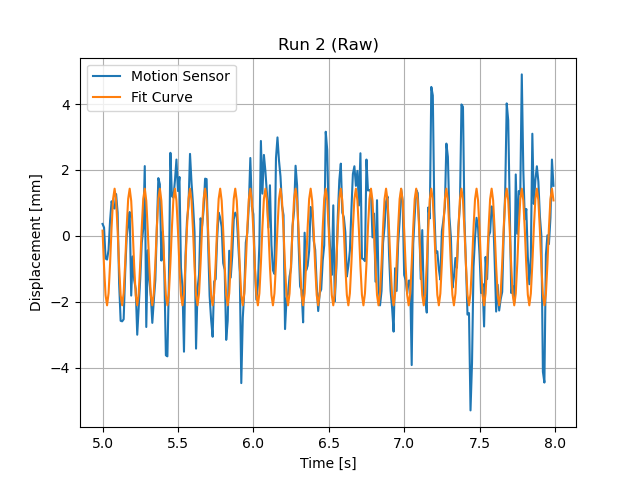
\includegraphics[width=1.0\textwidth]{images/Graphs/Run_2-Raw-Zoomed} % first figure itself
        \caption{Raw data from Test \num{2}, zoomed to only show \qtyrange{5}{8}{\s}.}
        \label{fig:run_2-raw-zoomed}
    \end{minipage}\hfill
    \begin{minipage}{0.45\textwidth}
        \centering
        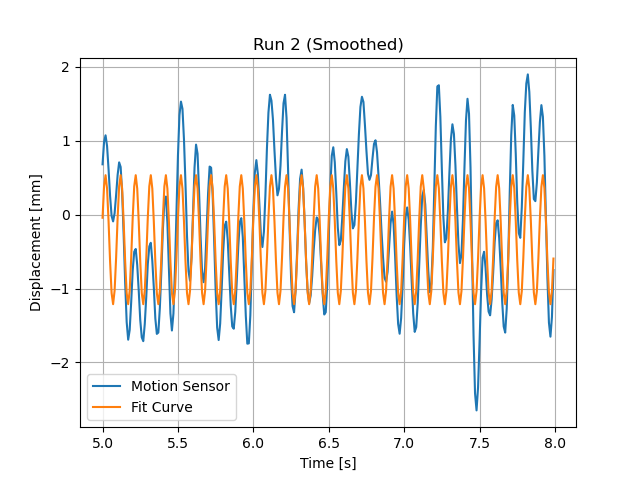
\includegraphics[width=1.0\textwidth]{images/Graphs/Run_2-Smoothed-Zoomed} % second figure itself
        \caption{Smoothed data from Test \num{2}, zoomed to only show \qtyrange{5}{8}{\s}.}
        \label{fig:run_2-smoothed-zoomed}
    \end{minipage}
\end{figure}

The line of best fit does not account for the secondary oscillations due to the hanging weight---it averages between the high and low secondary oscillations--but from looking at the motion sensor measurements shown in Figure \ref{fig:run_2-smoothed-zoomed}, you can observe the periods of oscillation where the weight was applying a downwards force on the beam, \eg from \qtyrange{5.2}{5.5}{\s}.

The equations of the lines of best for Figures \ref{fig:run_2-raw-zoomed} and \ref{fig:run_2-smoothed-zoomed} are given in Equations \ref{eqn:run_2-raw-lobf} and \ref{eqn:run_2-smoothed-lobf} respectively.

\begin{equation} \label{eqn:run_2-raw-lobf}
f(t)=-1.771\sin(62.83t-0.2651)-0.3391
\end{equation}

\begin{equation} \label{eqn:run_2-smoothed-lobf}
f(t)=0.8731\sin(62.83t+0.3724)-0.3387
\end{equation}

\subsection{Test 3} \label{data-test_3}
Shown in Figures \ref{fig:run_3-raw-zoomed} and \ref{fig:run_3-smoothed-zoomed} is the raw data and smoothed data respectively for Test \num{3}. At the beginning of this run, a force was applied to a weight hanging from a spring connected to the beam causing the weight to oscillate. At random times during the run, a member from our group applied an arbitrary impulse with their hand to the end of the beam (see Section \ref{procedures-test_3} for details).

The smoothed data was generated using a two-pass rolling mean algorithm. The first pass used a window of \num{5} and the second pass used a window of \num{3}.For clarity, only the data from \qtyrange{5}{8}{\s} is shown in Figures \ref{fig:run_3-raw-zoomed} and \ref{fig:run_3-smoothed-zoomed}.

\begin{figure}[htbp]
    \centering
    \begin{minipage}{0.45\textwidth}
        \centering
        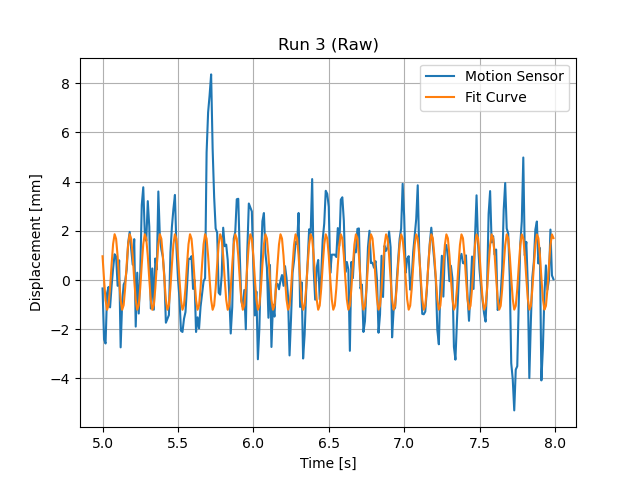
\includegraphics[width=1.0\textwidth]{images/Graphs/Run_3-Raw-Zoomed} % first figure itself
        \caption{Raw data from Test \num{3}, zoomed to only show \qtyrange{5}{8}{\s}.}
        \label{fig:run_3-raw-zoomed}
    \end{minipage}\hfill
    \begin{minipage}{0.45\textwidth}
        \centering
        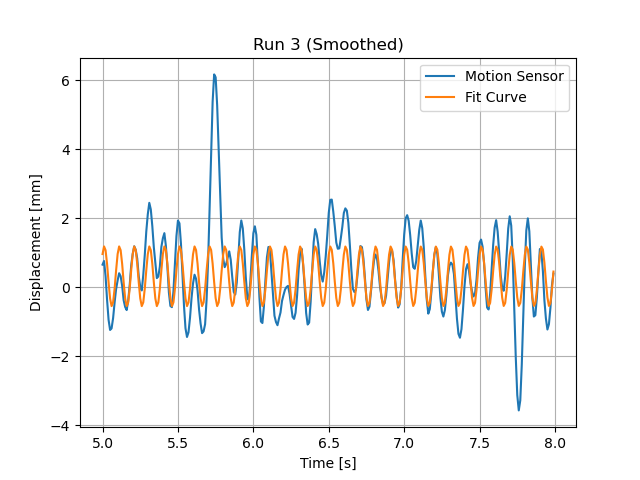
\includegraphics[width=1.0\textwidth]{images/Graphs/Run_3-Smoothed-Zoomed} % second figure itself
        \caption{Smoothed data from Test \num{3}, zoomed to only show \qtyrange{5}{8}{\s}.}
        \label{fig:run_3-smoothed-zoomed}
    \end{minipage}
\end{figure}

We observe from Figures \ref{fig:run_3-raw-zoomed} and \ref{fig:run_3-smoothed-zoomed} the same secondary oscillations we observed in Test \num{2} (Section \ref{data-test_2}. In addition to the secondary oscillations, we also note the large spikes at \qty{5.75}{\s} and \qty{7.75}{\s}. These spikes were due to the arbitrary impulses being applied to the beam by one of our group members.

The equations of the lines of best for Figures \ref{fig:run_3-raw-zoomed} and \ref{fig:run_3-smoothed-zoomed} are given in Equations \ref{eqn:run_3-raw-lobf} and \ref{eqn:run_3-smoothed-lobf} respectively.

\begin{equation} \label{eqn:run_3-raw-lobf}
f(t)=-1.547\sin(62.82t-0.3488)+0.3259
\end{equation}

\begin{equation} \label{eqn:run_3-smoothed-lobf}
f(t)=0.8700\sin(62.82t+0.9127)+0.3228
\end{equation}

\chapter{Conclusion} \label{conclusion-chapter}
\section{Analysis} \label{analysis}
\subsection{Test 1 and the Displacement Sensor} \label{analysis-test_1_and_the_displacement_sensor}
As described in Section \ref{procedures-test_1}, Test \num{1} was the only test to include the data from the displacement sensor. Figure \ref{fig:run_1-raw-zoomed} in Section \ref{data-test_1} clearly shows why the displacement sensor was inadequate for our purposes in this lab. To reiterate the excerpt from Section \ref{data-test_1}:

\begin{displayquote}
From these graphs, it is clear the displacement sensor's polling rate was too slow. In retrospect, the reason is clear. As shown from Figure \ref{fig:run_1-smoothed-zoomed} and as described in Section \ref{procedures-setup}, the wave driver was forcing the beam to oscillate at a rate of approximately \qty{10}{\hertz}, but the polling rate of the displacement sensor was \qty{5}{\hertz}. In other words, the resolution of the displacement sensor was too low to accurately measure the true displacement of the beam. For this reason, the displacement sensor was omitted from the second and third tests.
\end{displayquote}

The motion sensor, however, is a much more precise measurement tool. From the smoothed data in Figure \ref{fig:run_1-smoothed-zoomed}, it is possible to count the number of cycles that occur in one second, and if done correctly, you will find there almost exactly \num{10} cycles each second. The line of best fit---which may not excel at matching the sinusoidal center at any given time---from the raw data in \ref{fig:run_1-raw-zoomed} correctly estimates the frequency of the beam's displacement to be \qty{9.999}{\hertz} (see Appendix \ref{output} for full script output). This quantitative result matches the qualitative counting result, confirming that even despite the noise and variation in sinusoidal center, the beam was indeed oscillating at \qty{10}{\hertz} as expected, and the motion sensor was correctly recording the oscillations.

\subsection{Data Processing} \label{analysis-data_processing}
A detailed discussion of how we smoothed the data and generated the line of best fit can be found in Section \ref{data}. We used multi-pass rolling mean algorithms to smooth the data with assistance from the \texttt{pandas} Python library. When attempting to generate the line of best fit, we had troubles using the \texttt{scipy.optimize()} function. It seemed that the subtle variations in frequency due to the external forces being applied or even just stray vibrations in the apparatus were enough for the \texttt{scipy.optimize()} function to fail.

The solution---which is described in more detail in Section \ref{data}---was to use a Fast Fourier Transformation algorithm to predict the frequency of the data, and then to use the \texttt{scipy.{\allowbreak}optimize()} function to optimize the sine curve parameters. This method turned out to be quite successful, and despite the variations in the sinusoidal center, the line of best fit matches the peaks and troughs of the actual data well.

In Tests \num{2} and \num{3}, the spring-weight mechanism (see Sections \ref{apparatus}, \ref{procedures-test_2}, and \ref{procedures-test_3}) caused a secondary sinusoidal oscillation, proportional to the oscillation of the spring-weight system. This secondary oscillation caused the data to deviate from the line of best by changing the sinusoidal center of the data. If we had more time, we would have liked to modify the line of best function to include a second sine term in the optimized function.

Additionally, in Test \num{3}, the random impulses applied by one of our group members showed up clearly in the data as discussed in Section \ref{data-test_3}. They significantly deviate from the line of best fit and despite the smoothing, it is still evident they were the result of an external impulse and not just erroneous measurements.

In Tests \num{1} and \num{2}, the line of best fit for the raw data estimated the sinusoidal center to be less than zero. This was confusing initially, but upon further inspection we realized this was a reasonable result. In a vacuum with no gravitational influence, if a downward force were applied to the beam, and the beam reacted perfectly elastically to the deformation, the beam would oscillate exactly around the point of zero displacement. This experiment did not take place in a zero-gravity vacuum; so, we can assume the reason the sinusoidal center was below zero was due to gravity, air resistance, and energy loss due to vibrations in the apparatus.

Lastly, in Test \num{1}, the graph of the full raw data shows large variations in the amplitude and sinusoidal center of the displacement curve. We were unable to come up with a strong explanation; however, we hypothesized that the reason could have been due to the small downward force being applied by the displacement sensor ``needle''. The force of this needle was certainly slight, but the displacements being recorded were generally \qty{5}{\mm} or less, \ie even a small force is not negligible at this scale.

\subsection{Sources of Error} \label{analysis-sources_of_error}
In our experiments, we identified the following potential sources of error:

\begin{itemize}
	\item The slight downward force of the displacement sensor ``needle'' could have absorbed some of the elastic energy generated by the wave driver displacing the beam. This would push the sinusoidal center of the displacement data lower than it should be.
	\item The PASCO tool kit sensors were zeroed before each test; however, its possible the instruments were bumped slightly while starting the test or jostled by the forces and vibrations of the wave driver. Additionally, after many uses, the measurement devices could be miscalibrated.
	\item The styrofoam reflector piece that was taped to the bottom of the beam was slightly loose, and if the reflector plate was rotating slightly or not staying flush to the beam, the result would be small errors in the displacement of the beam.
	\item The tautness of the string was checked qualitatively, and if the string were over or under-tightened, this would affect the amount of elastic energy being imparted on the beam.
\end{itemize}

In a real airplane, there are myriad forces battering the airplane at any point in time. The regular turbulence of the air in higher altitudes, strong gusts of wind or storms, or pockets of variable air pressure could all explain the spikes shown in Test \num{3}. The secondary oscillation we observed in Test \num{2} and \num{3} could also be explained by a combination of vibrations: aerodynamically related vibrations coupled with strong internal vibrations such as that of the jet engines or motors. Even loose control surfaces or objects obstructing airflow over the skin of the plane could contribute to the type of oscillations we observed in our representative tests.

\section{Conclusion} \label{conclusion-section}
After analyzing all the data, our hypotheses in Section \ref{hypothesis} generally held true, the most notable exception being our hypothesis of Test \num{1} (Section \ref{hypothesis-test_1}. We expected the data to look much cleaner, but even in the simplest apparatus configuration, there was considerable noise and variation in the recorded data.

This was an important lesson to learn: when measuring at such a precise scale, it is imperative to practice good data processing techniques. We also learned it is important to choose the correct measuring device. The displacement sensor was totally incapable of properly recording the displacement of the beam, but if we had not also used the motion sensor to record the beam deflection, it may have been hard to identify that the displacement sensor was the source of the ``biased'' error.

\printbibliography[heading=subbibintoc]

\appendix
\chapter{Graphs} \label{graphs}
\section{Regular LOBF Graphs} \label{regular_lobf_graphs}

% TEST 1 GRAPHS

\begin{figure}[htbp]
\centering
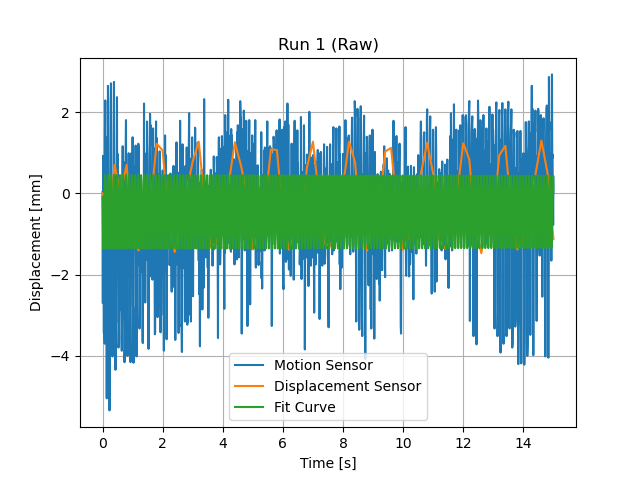
\includegraphics[width=4in]{images/Graphs/Run_1-Raw}
\caption{Raw data from Test \num{1}.}

\centering
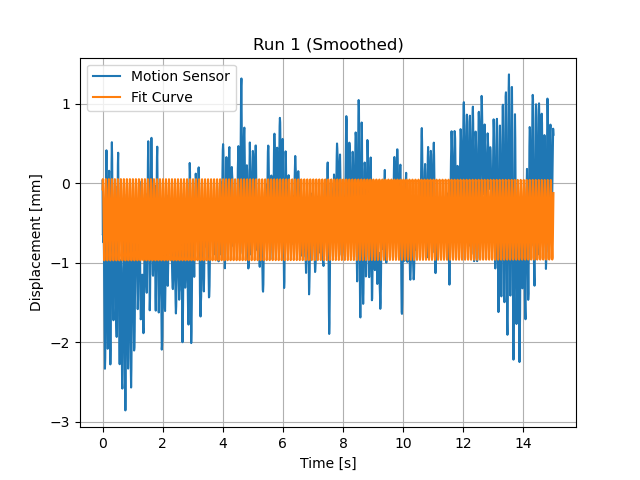
\includegraphics[width=4in]{images/Graphs/Run_1-Smoothed}
\caption{Smoothed data from Test \num{1}.}
\end{figure}

\begin{figure}[htbp]
\centering
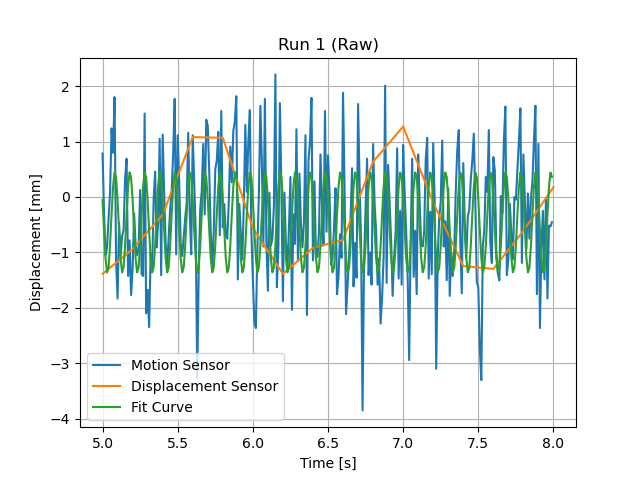
\includegraphics[width=4in]{images/Graphs/Run_1-Raw-Zoomed}
\caption{Raw data from Test \num{1}, zoomed to only show \qtyrange{5}{8}{\s}.}
\end{figure}

\begin{figure}[htbp]
\centering
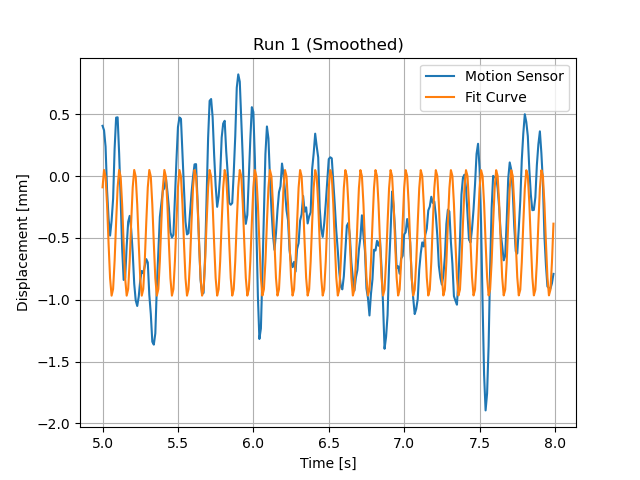
\includegraphics[width=4in]{images/Graphs/Run_1-Smoothed-Zoomed}
\caption{Smoothed data from Test \num{1}, zoomed to only show \qtyrange{5}{8}{\s}.}
\end{figure}

% TEST 2 GRAPHS

\begin{figure}[htbp]
\centering
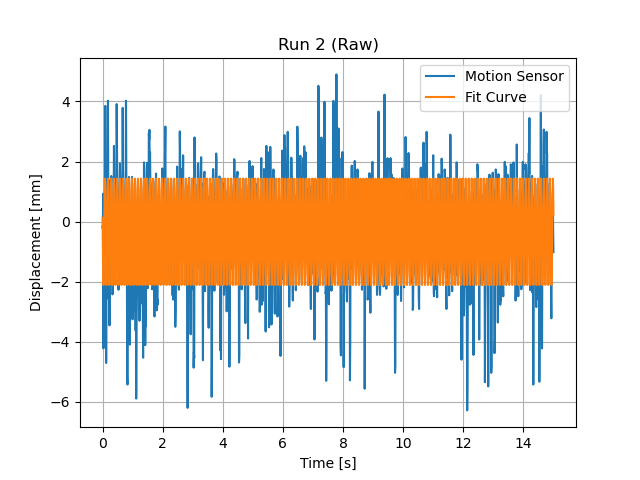
\includegraphics[width=4in]{images/Graphs/Run_2-Raw}
\caption{Raw data from Test \num{2}.}
\end{figure}

\begin{figure}[htbp]
\centering
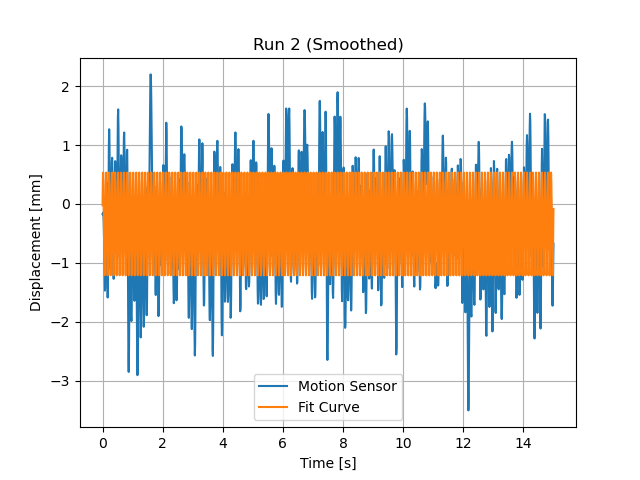
\includegraphics[width=4in]{images/Graphs/Run_2-Smoothed}
\caption{Smoothed data from Test \num{2}.}
\end{figure}

\begin{figure}[htbp]
\centering
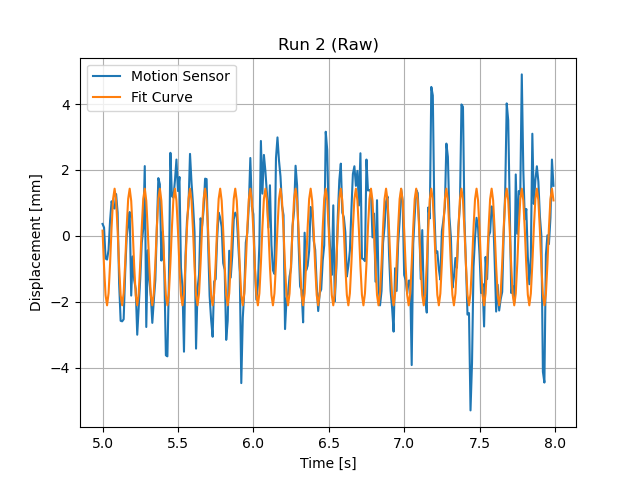
\includegraphics[width=4in]{images/Graphs/Run_2-Raw-Zoomed}
\caption{Raw data from Test \num{2}, zoomed to only show \qtyrange{5}{8}{\s}.}
\end{figure}

\begin{figure}[htbp]
\centering
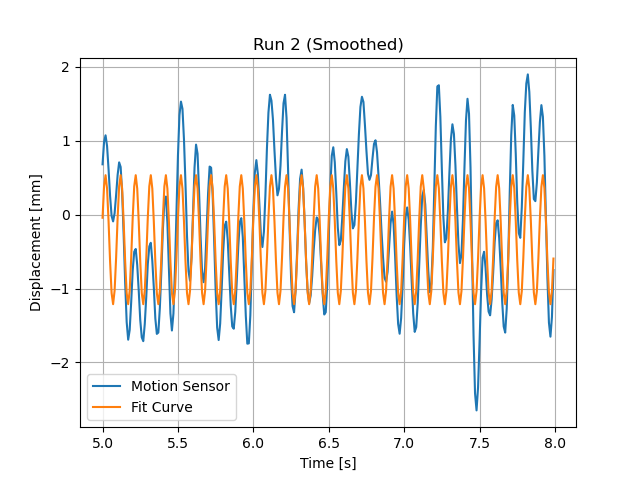
\includegraphics[width=4in]{images/Graphs/Run_2-Smoothed-Zoomed}
\caption{Smoothed data from Test \num{2}, zoomed to only show \qtyrange{5}{8}{\s}.}
\end{figure}

% TEST 3 GRAPHS

\begin{figure}[htbp]
\centering
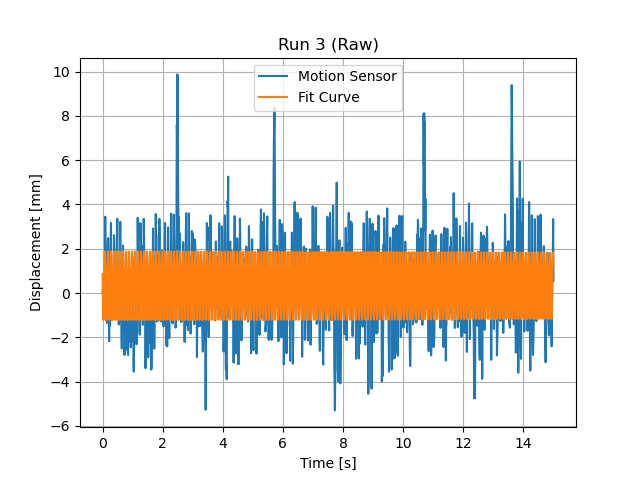
\includegraphics[width=4in]{images/Graphs/Run_3-Raw}
\caption{Raw data from Test \num{3}.}
\end{figure}

\begin{figure}[htbp]
\centering
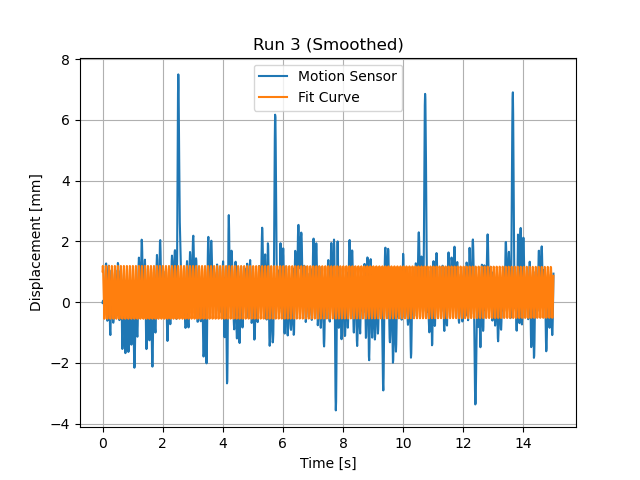
\includegraphics[width=4in]{images/Graphs/Run_3-Smoothed}
\caption{Smoothed data from Test \num{3}.}
\end{figure}

\begin{figure}[htbp]
\centering
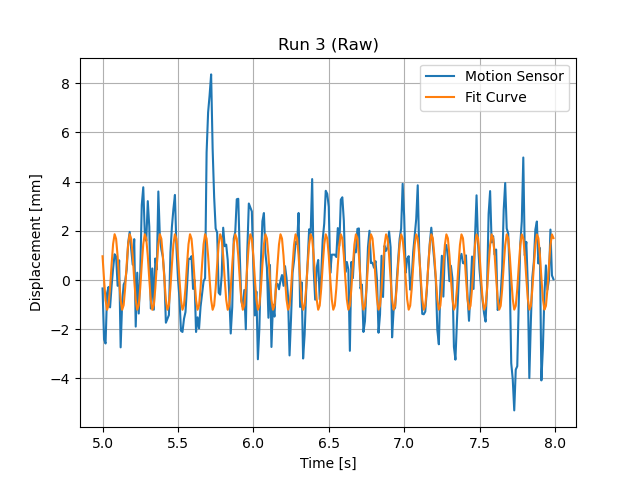
\includegraphics[width=4in]{images/Graphs/Run_3-Raw-Zoomed}
\caption{Raw data from Test \num{3}, zoomed to only show \qtyrange{5}{8}{\s}.}
\end{figure}

\begin{figure}[htbp]
\centering
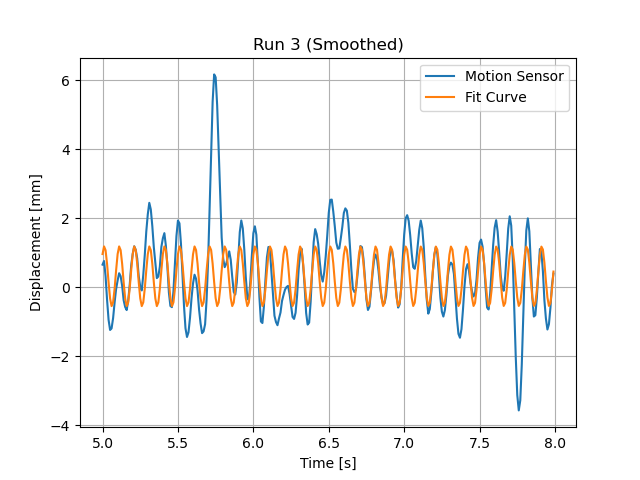
\includegraphics[width=4in]{images/Graphs/Run_3-Smoothed-Zoomed}
\caption{Smoothed data from Test \num{3}, zoomed to only show \qtyrange{5}{8}{\s}.}
\end{figure}

\newpage
\section{Piece-Wise LOBF Graphs} \label{piece-wise_lobf_graphs}

% TEST 1 GRAPHS

\begin{figure}[htbp]
\centering
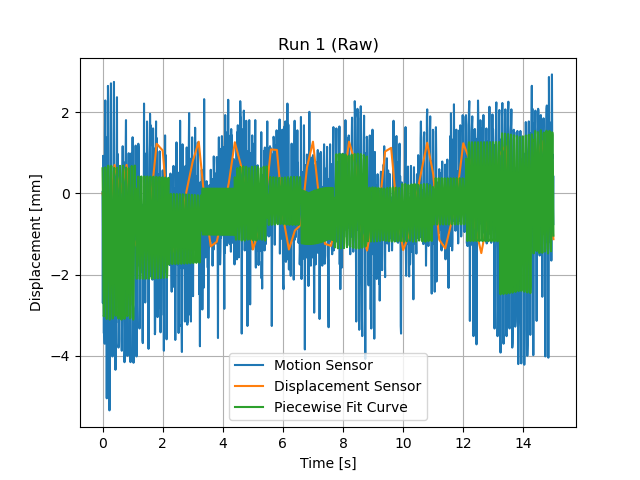
\includegraphics[width=4in]{images/Graphs/Run_1-Raw-PW}
\caption{Raw data from Test \num{1}. Uses the piece-wise line of best fit.}

\centering
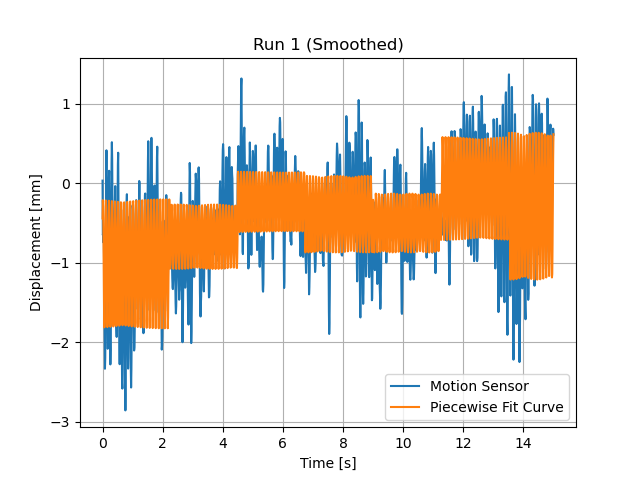
\includegraphics[width=4in]{images/Graphs/Run_1-Smoothed-PW}
\caption{Smoothed data from Test \num{1}. Uses the piece-wise line of best fit.}
\end{figure}

\begin{figure}[htbp]
\centering
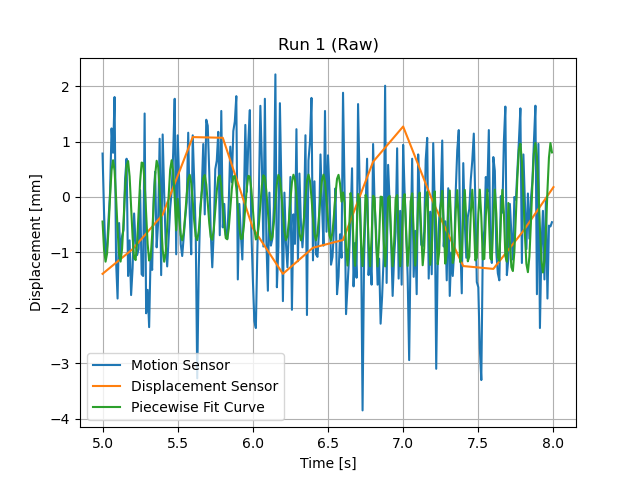
\includegraphics[width=4in]{images/Graphs/Run_1-Raw-PW-Zoomed}
\caption{Raw data from Test \num{1}, zoomed to only show \qtyrange{5}{8}{\s}. Uses the piece-wise line of best fit.}
\end{figure}

\begin{figure}[htbp]
\centering
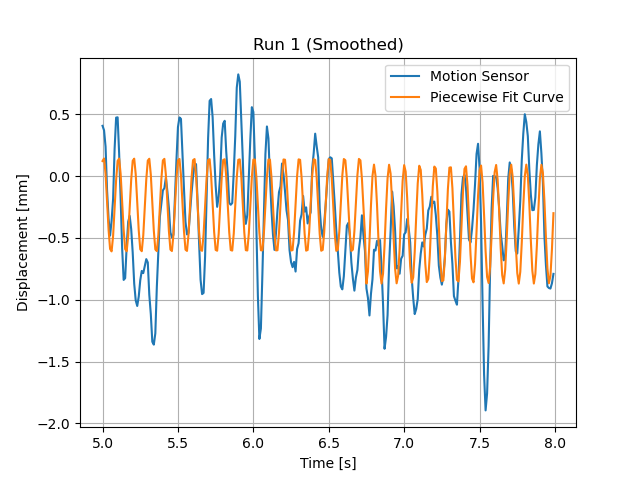
\includegraphics[width=4in]{images/Graphs/Run_1-Smoothed-PW-Zoomed}
\caption{Smoothed data from Test \num{1}, zoomed to only show \qtyrange{5}{8}{\s}. Uses the piece-wise line of best fit.}
\end{figure}

% TEST 2 GRAPHS

\begin{figure}[htbp]
\centering
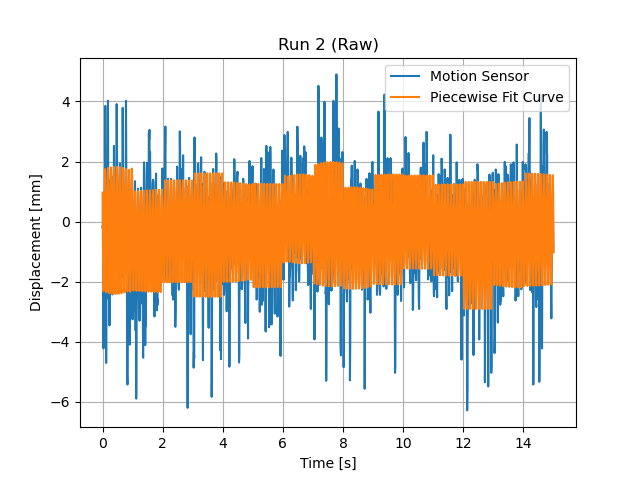
\includegraphics[width=4in]{images/Graphs/Run_2-Raw-PW}
\caption{Raw data from Test \num{2}. Uses the piece-wise line of best fit.}
\end{figure}

\begin{figure}[htbp]
\centering
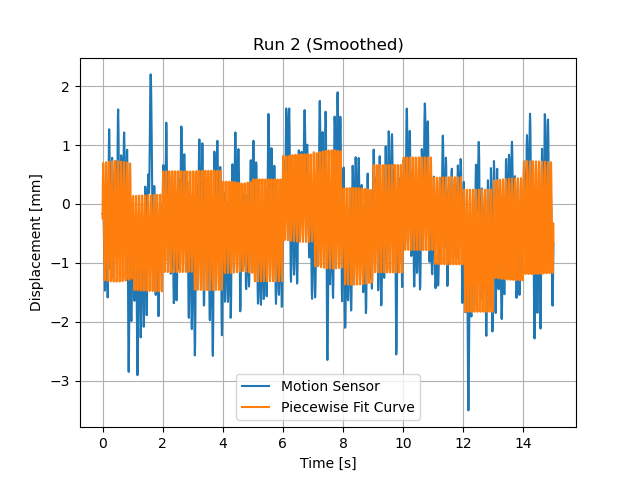
\includegraphics[width=4in]{images/Graphs/Run_2-Smoothed-PW}
\caption{Smoothed data from Test \num{2}. Uses the piece-wise line of best fit.}
\end{figure}

\begin{figure}[htbp]
\centering
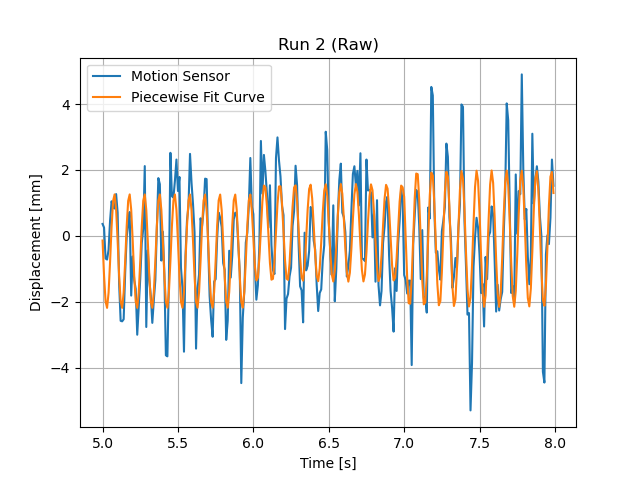
\includegraphics[width=4in]{images/Graphs/Run_2-Raw-PW-Zoomed}
\caption{Raw data from Test \num{2}, zoomed to only show \qtyrange{5}{8}{\s}. Uses the piece-wise line of best fit.}
\end{figure}

\begin{figure}[htbp]
\centering
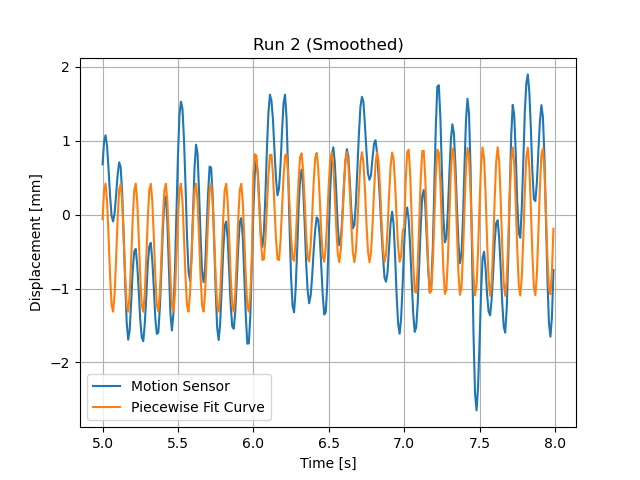
\includegraphics[width=4in]{images/Graphs/Run_2-Smoothed-PW-Zoomed}
\caption{Smoothed data from Test \num{2}, zoomed to only show \qtyrange{5}{8}{\s}. Uses the piece-wise line of best fit.}
\end{figure}

% TEST 3 GRAPHS

\begin{figure}[htbp]
\centering
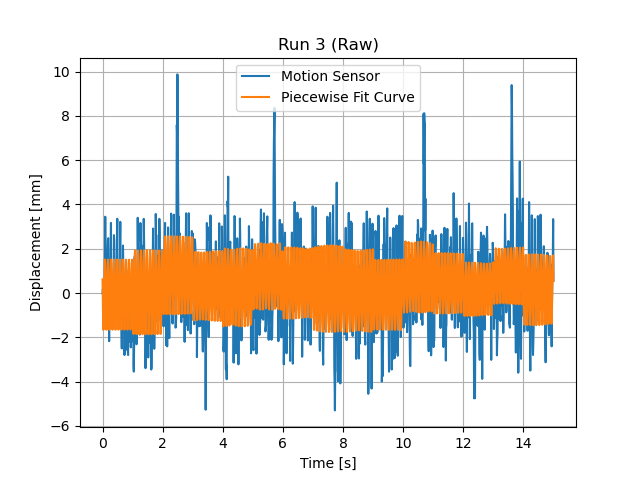
\includegraphics[width=4in]{images/Graphs/Run_3-Raw-PW}
\caption{Raw data from Test \num{3}. Uses the piece-wise line of best fit.}
\end{figure}

\begin{figure}[htbp]
\centering
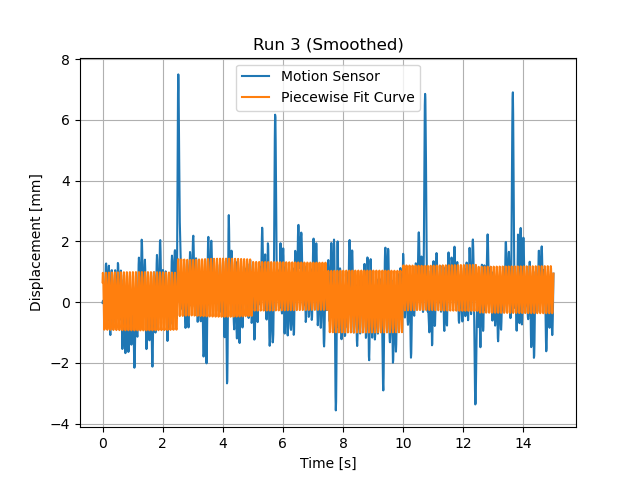
\includegraphics[width=4in]{images/Graphs/Run_3-Smoothed-PW}
\caption{Smoothed data from Test \num{3}. Uses the piece-wise line of best fit.}
\end{figure}

\begin{figure}[htbp]
\centering
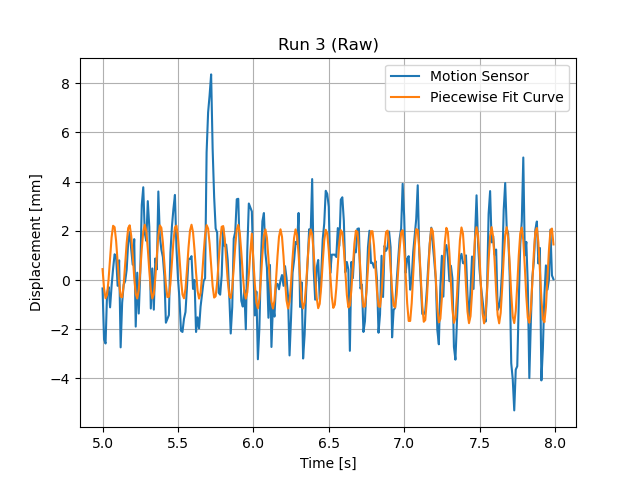
\includegraphics[width=4in]{images/Graphs/Run_3-Raw-PW-Zoomed}
\caption{Raw data from Test \num{3}, zoomed to only show \qtyrange{5}{8}{\s}. Uses the piece-wise line of best fit.}
\end{figure}

\begin{figure}[htbp]
\centering
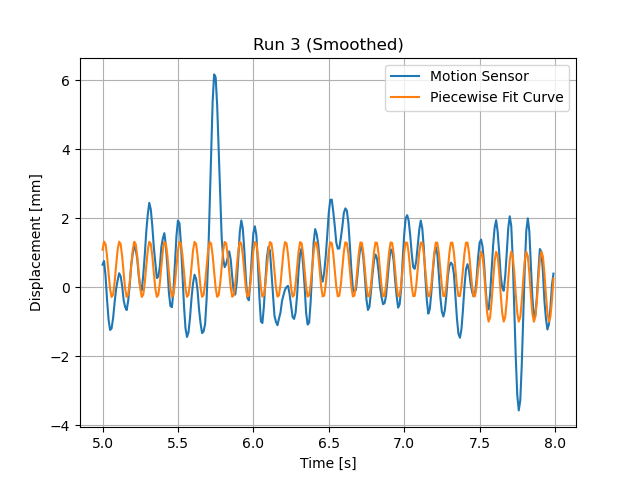
\includegraphics[width=4in]{images/Graphs/Run_3-Smoothed-PW-Zoomed}
\caption{Smoothed data from Test \num{3}, zoomed to only show \qtyrange{5}{8}{\s}. Uses the piece-wise line of best fit.}
\end{figure}

\chapter{Code} \label{code}

\section{Lab-01-Analysis.py} \label{lab-01-analysis.py}
\lstinputlisting[caption={Our data analysis script, \texttt{Lab-01-Analysis.py}.},language=Python]{src/Lab-01-Analysis.py}

\section{Output} \label{output}
\begin{verbatim}
Amplitude: -0.911702 mm
Frequency: 9.99878 Hz
LOBF: f(t) = -0.911702sin(62.8242 * t + -0.423851) + -0.458014
----------------------------------------------------------
Amplitude: 0.513407 mm
Frequency: 9.99862 Hz
LOBF: f(t) = 0.513407sin(62.8232 * t + 0.842215) + -0.459104
----------------------------------------------------------
Amplitude: -1.77111 mm
Frequency: 9.99939 Hz
LOBF: f(t) = -1.77111sin(62.828 * t + -0.26507) + -0.339128
----------------------------------------------------------
Amplitude: 0.873077 mm
Frequency: 9.99919 Hz
LOBF: f(t) = 0.873077sin(62.8267 * t + 0.372368) + -0.338719
----------------------------------------------------------
Amplitude: -1.54725 mm
Frequency: 9.99753 Hz
LOBF: f(t) = -1.54725sin(62.8163 * t + -0.348804) + 0.325918
----------------------------------------------------------
Amplitude: 0.870026 mm
Frequency: 9.99747 Hz
LOBF: f(t) = 0.870026sin(62.816 * t + 0.912736) + 0.322807
----------------------------------------------------------
Max Displacement of Run 1: -5.3458 mm or 2.9268 mm
Max Displacement of Run 2: -6.2847 mm or 4.9003 mm
Max Displacement of Run 3: -5.3 mm or 9.8693 mm
\end{verbatim}

\end{document}
